%10
\documentclass[output=paper]{LSP/langsci}
\author{David Rood}
\title{The phonology of {Lakota} voiced stops}


\abstract{Lakota has two phonetic voiced stops, [b] and  [g], which do not behave like stops. They occur in \isi{cluster}s with \isi{sonorant}s, and in syllable or morpheme final position as the result of several morphophonemic processes. In the \isi{cluster}s, their behavior is easily described using the distinctive feature [\textsc{sonorant voice}] proposed in \citet{Rice1993}, but in coda\is{coda position} position they (and the fricatives, and the lateral sonorant [l]) manifest \isi{lenition} instead. In this lenition environment, both voicing and \isi{nasalization} are variable, leading to the proposal that Lakota is an \isi{aspiration language} like English rather than a voicing language like French. 
% KEYWORDS: [Lakota, voicing, voiced stop, sonorant voice, lenition]
}
\ChapterDOI{10.17169/langsci.b94.173}

\maketitle

\begin{document}

Look at almost any written \ili{Lakota} text or \isi{dictionary}, and you will see many instances of the letters <b> and <g>. Look at any \ili{Lakota} grammar, and you will learn that these letters (for the most part) do not represent contrastive sounds in the language --- they represent allophones of /p/ or /ph/ and /k/ respectively. Yet everyone who writes the language uses both <b> and <g> to some extent, so they must seem salient to those who speak, study or record the language. What is their status, really?
 
To investigate this question, the following discussion will call on phonological theory (particularly \isi{autosegmental phonology} and \isi{feature geometry}; see \citealt{Clements1985}), the concept of two kinds of phonological [\textsc{voice}] features (\citealt{Rice1993}), the \isi{typology} of the way languages realize the feature [\textsc{voice}] (i.e. the difference between \isi{aspiration language}s and voicing languages -- \citealt{RingenEtAl2013}), and the history of the language. Also relevant, it turns out, are some of the unusual properties of the feature [\textsc{nasal}] in this language (and in Siouan in general). Combining these tools gives us a consistent picture of how these voiced stops function in \ili{Lakota}: they are sonorants, or more precisely, \isi{sonorant obstruents}, in an \isi{aspiration language}. \citet{Rankin2001}, an unpublished conference paper, examined much of the same data and came to similar conclusions based on historical and comparative\is{comparative method} evidence and argumentation. I will try to summarize his arguments in parallel with mine in what follows. 

\section{Orthographic and structural preliminaries}

Before tackling the investigation, however, we need some facts about \ili{Lakota} and its \isi{orthography} in order to understand the data. All examples are presented in the \isi{orthography} of the \textit{New \ili{Lakota} Dictionary\is{dictionary}} (\citealt{Ullrich2012}), with the modification that we sometimes need to use <ʔ> to illustrate a point. The \ili{Lakota} consonant inventory is presented in this \isi{orthography} in Table 1. The table shows only one category of aspirated stops, however, though the language uses two kinds of aspiration that are not quite in complementary distribution. Aspiration on stops may therefore sometimes be represented by <\v{h}> instead of <h>. Likewise not shown in this table is the symbol <ŋ>, which marks \isi{nasalization} of a preceding vowel. Occasionally, however, we need to represent phonetically the velar nasal for which the IPA symbol is exactly this one. In those cases, the symbol is enclosed in square brackets, viz. [ŋ].

Another important feature of the presentation of the examples is the so-called ablauting vowel. Some \ili{Lakota} verbs change their final vowel in certain grammatical contexts. The options are [a, aŋ, e, iŋ]. To indicate that an example is a verb from this category, it is traditional in \ili{Lakota} lexicography to present the word with the final vowel <A> or <Aŋ>.

We will sometimes have occasion to cite reduplicated forms in what follows. The syllable which is copied cannot be predicted for most words, and whether the copied syllable is inserted before or after its model is also variable.

Finally, since we are discussing phenomena that are only marginally phonemic, if at all, we will often need to indicate the systematic status of a consonant. I have used the traditional slashes (/.../) for underlying or phonemic sounds, and square brackets ([...]) for actual pronunciations. In \tabref{consonantinventory}, (ʔ) represents the \isi{glottal} stop, which the standard \isi{orthography} assumes is predictable between vowels and optional in word-initial position, but which may sometimes be structurally important, if not actually phonemic, in morpheme-initial position, as we will see below. Letters in angle brackets (<...>) are letters, not sounds.

\begin{table}[tbp]
\caption{\ili{Lakota} consonant inventory using the standard \isi{orthography}}\label{consonantinventory}
\begin{tabular}[t]{ c  c  c  c  c  c }
\lsptoprule 
 & Labial & Alveolar & Alveo-palatal & Velar & Laryngeal\\
\midrule
Unaspirated stop\is{simple stops}  & p & t & \v{c} & k & (ʔ)\\
or affricate & & & & & \\
 
Ejective\is{ejective} & p' & t' & \v{c}' & k' & \\
 
Aspirated & ph & th & \v{c}h & kh &\\
 
Voiced stop & b & & & g &\\
 
Voiceless \isi{fricative} & & s & \v{s} & \v{h} &\\
 
Voiced \isi{fricative} & & z & \v{z} & \v{g} &\\
 
Lateral & & l & & &\\
 
Nasal & m & n & & &\\
 
Glide & w & & y & & h\\
\lspbottomrule
\end{tabular}
\end{table}

\section{The patterns}

The letters we want to study are of course meant to indicate voiced stops. They occur in two patterns: as the first members of \isi{cluster}s, and in morpheme final position when an underlying morpheme final vowel is lost. The loss of the vowel restructures the syllables of the word, putting the formerly preceding consonant into the \isi{coda position} of the formerly penultimate syllable.

\subsection{The distribution of the voiced stops}

\subsubsection{[b]}

The stops in question occur both singly and in \isi{cluster}s. The only \isi{cluster} including [b] is [bl], but it enjoys very high frequency because it is the first-person agent marker for the large number of common verbs which begin with /y/ (the [l] replaces the /y/). Singly, the sound represented by the letter <b> occurs contrastively in just one borrowed word, one probably onomatopoetic word, three roots, and one conjugated verb:\footnote{Thanks to the anonymous reviewer for reminding me of some of these.}

\begin{exe} \label{ex:rood:1}
\ex Words with phonemic /b/
\begin{xlist}
\ex \textit{bébela} `baby'
\ex \textit{\v{s}kíbibila}`black capped chickadee'
\ex \textit{bá} `to blame' (not widely known)
\ex \textit{ábela} `scattered' (with several derivations)
\ex \textit{kabú} `to play the drum' (\textit{ka-} `by hitting'; \textit{bu} `make a hollow noise')
\ex \textit{wahíbu} `I left to come' (archaic) \textit{wa} `I'; \textit{hiyu} `to start coming'; \textit{y>b} `I')
\end{xlist}
\end{exe} 

The borrowed word, presumably from \ili{French}, is \textit{bébela} `baby' (\textit{-la} is the regular \ili{Lakota} diminutive). The possibly onomatopoetic bird name, \textit{\v{s}kíbibila}, is also recorded \textit{\v{s}kípipila}, and the form with the plain voiceless stop is actually the preferred one, according to the \isi{dictionary}. The roots are \textit{bá} `to blame, to criticize', \textit{-be-}, found only in adverbs having to do with being scattered, and \textit{bú} `to make a loud, hollow noise'. The first is seldom used; the second is also recorded \textit{pe} in the older Buechel \isi{dictionary} (\citealt[278]{Buechel1970} under the entry \textit{kaibebekiya}); and the last is used with several derivational prefixes such as \textit{ka-} `by hitting' in \textit{kabú} `to play the drum'. Formerly, [b] also occurred as part of the first-person agent marking for the verb \textit{hiyú} `to start coming', which used to be doubly conjugated, \textit{wahíbu}; today the form is regularized to \textit{wahíyu}.

\citet[8]{Rankin2001} asserts that [b] is a regular allophone of /w/ in that only the former occurs before /u/: we have syllables [wi], [we], [wa], [wo], but [bu]. However, he gives no examples of this [bu], only examples of \isi{cluster}s ending in /w/ (gwu, swu, \v{s}wu, \v{h}wu) where the first element of the \isi{cluster} prevents the allophone rule from applying.\footnote{In the closely related \ili{Dakota} dialect\is{dialects}, the behavior of sonorants is different from what we find in \ili{Lakota}. For example, the \isi{cluster}s /sw/, etc. are [sb] etc. there. I do not know whether [b] or [w] is older. Although the reviewer suggested I discuss the \ili{Dakota} patterns as well, it seems to me they are different enough to provide more distraction than enlightenment. For example, corresponding to \ili{Lakota} [gl] we find \ili{Dakota} [hd]. There is a long and complicated debate in the phonological literature over whether or not [h] is a \isi{sonorant}, to which these \ili{Dakota} data can contribute, but that is a topic for another paper.} The anonymous reviewer for this chapter also pointed out that [b] occurs in some \isi{compound}s where we expect [bʔ]. The example cited is \textit{hítobuya} `four-year-old calf or colt' contracted from \textit{t\'opa} `four' and \textit{ʔuyÁ} `to grow'. The voiced stop is expected if the \isi{glottal} stop is pronounced, and sometimes voicing remains even if the \isi{glottal} stop is lost. Cf. discussion of the interaction of voiced stops with \isi{glottal} stops in \S 4.2 below.

In all its other occurrences, [b] is in complementary distribution with /p/ and /ph/. In what follows, I will ignore phonemic /b/ (in words like those in example \REF{ex:rood:1}), since it does not alternate with anything and can be considered an ordinary voiced obstruent. The feature [\textsc{laryngeal voice}] is at work here as it is with the fricatives.

We will also see that the [bl] \isi{cluster} can absorb \isi{nasalization} from a following vowel and become [mn], another phenomenon that we need to account for.

\subsubsection{[g]} 
\largerpage
The sound represented by <g> is a little different. It is never contrastive, and in non-morpheme-final contexts we find the \isi{cluster}s [gl, gw, gm] and [gn]. A reviewer for this volume as a whole pointed out that there are also examples of the \isi{cluster} [g\v{z}] in reduplications where the [g] represents an underlying /l/, following a pattern known as coronal dissimilation discovered by \citet[225--226]{Carter1974} and also discussed by \citet[338]{Shaw1980}.  Since this [g] presumably inherits its voice from the underlying /l/, the voicing here must be [\textsc{SV}].  See examples in \REF{ex:rood:2}, with the reduplication enclosed in angle brackets.
 

\begin{exe}
\ex\label{ex:rood:2}
 \begin{xlist}
\ex \textit{waŋ<\v{z}íg>\v{z}ila} `one at a time' (reduplication of \textit{waŋ\v{z}íla} `one')
\ex \textit{o<\v{z}úg>\v{z}ula} `several to be full', reduplication of \textit{o\v{z}úla} `to be full')
\end{xlist}
\end{exe}

Neither [k] nor [kh] ever occurs in obstruent-\isi{sonorant} \isi{cluster}s. 

Another difference between [g] and [b] is that for unknown reasons [g] never nasalizes\is{nasalization} in  \isi{cluster}s, though /l/ may, changing [gl] to [gn]. Both [gl] and [gn] are frequently the result of a /k/ morpheme occurring before and combining with an initial /y/ of a verb.

\begin{exe}
\ex \label{ex:rood:3}
Examples of the \isi{cluster}s beginning with [g] and [b]
\begin{xlist}
\ex \textit{Oglála} `Oglala'
\ex \textit{wagmú} `squash', lit. 'curved thing' (\textit{wa-} `indefinite patient'; \\	\textit{gmu} `curved')
\ex \textit{gnáyaŋ} `to fool, play tricks on, deceive'
\ex \textit{yugwá} `to shell, as corn; to open vegetable pods' (\textit{yu-} `by hand'; \\ \textit{gwa} `??')
\ex \textit{obláye} `prairie'
\ex \textit{waŋblí} `eagle'
\ex \textit{blé} `lake'
\end{xlist}
\end{exe}

\subsection{Fricatives}

As we saw in Table 1, both voiced and voiceless fricatives are phonemic. Examples are in \REF{ex:rood:4}. This voice contrast is not reconstructable to \ili{Proto-Siouan}, but is limited to the Central Siouan\il{Mississippi Valley Siouan} languages. Exactly how it arose is unknown. \citet{Miner1979a} pointed out that voiced stops and voiceless fricatives form a single phonological class in \ili{Dakotan}, \ili{Dhegiha}, \ili{Ho-Chunk} and \il{Ioway, Otoe-Missouria}Chiwere (i.e. all the Central Siouan\il{Mississippi Valley Siouan} languages) for purposes of forming \isi{cluster}s with sonorants.

\begin{exe}
\ex \label{ex:rood:4}
Voice contrasts in \ili{Lakota} \isi{fricative}s
\begin{xlist}
\ex \textit{zí} `yellow' vs. \textit{sí} `foot'
\ex \textit{\v{g}ú} `burned' vs. \textit{\v{h}é} `mountain'
\ex \textit{waŋ\v{z}í} `one' vs. \textit{wa\v{s}í} `I ordered him to'
\end{xlist}
\end{exe}

\citet[4]{Rankin2001} summarizes what I, too, believe about the fricatives:

\begin{quote}The underlying status of \ili{Dakotan} root-final \isi{fricative}s has received a lot of, in my opinion, undeserved attention in the literature. \ili{Proto-Siouan}, as far as we can tell, had only voiceless \isi{fricative}s. Present-day voiced \isi{fricative}s have several sources, not all of them regular, for example the initial /z/ of záptaŋ `five' which corresponds with /s/ virtually everywhere else in Siouan. The definitive study of voiced \isi{fricative} origins has yet to be done. One of the primary sources of voiced fricatives in \ili{Mississippi Valley Siouan} languages including \ili{Dakota} seems to have been post-accentual voiceless fricatives, i.e.,\vspace{-1em}
\begin{center}
s \v{s} \v{h} > z \v{z} \v{g} / V$'$  \underline{\hspace{1em}}
\end{center}
\vspace{-1em}
It is the case, however, that for one reason or another, voiced and voiceless \isi{fricative}s do contrast in this environment, so, underlyingly, I would leave the fricatives as they are on the surface. In any event, the fricatives in and of themselves do not present any special problems; even if we consider them underlyingly voiced, as do Carter\ia{Carter Jr., Richard~T.} and, at least originally, Shaw\ia{Shaw, Patricia~A.}, we simply posit a syllable-final (also word-final) devoicing rule of the sort familiar from \ili{German}, \ili{Russian} and a host of other garden variety languages. Syllable-final devoicing is also extremely common --- only slightly less so than word-final devoicing. So much for the fricatives: they merely do what is expected of obstruents. The real problem is the stops anyway.\end{quote}

\subsection{Morpheme-final position or coda position\is{coda position}}

\ili{Lakota} nouns and verbs always end in a vowel in their underlying forms. However, there are some very frequently occurring contexts in which the final vowel is lost, often indicating a subordinate\is{subordination} or dependent relationship with a following word, or simply as a consequence of fast speech. When the vowel is lost, the consonant preceding it changes in systematic ways: voiced \isi{fricative}s are devoiced, as we just learned, and labial and velar stops are at least partially voiced. The coronal stop /t/ becomes [l], and the coronal affricate, /\v{c}/, changes either to [l] or to [g] depending on the word. Often roots ending with /\v{c}/ have some consonant final forms with [l] and others with [g] (see \REF{ex:rood:5}). In what follows, we will try to show that these changes are all manifestations of a single process: morpheme- or syllable-final \isi{lenition}.

\begin{exe}
\ex\label{ex:rood:5}
Variable (lexically conditioned) change in morpheme-final /\v{c}/
\begin{xlist}
\ex \textit{\v{s}í\v{c}A} `bad' reduplicates as \textit{\textbf{\v{s}ig}\v{s}í\v{c}a}
\ex \textit{\v{s}i\v{c}A} `bad' + \textit{yá} 'causative' > \textit{\textbf{\v{s}il}yá}
\end{xlist}
\end{exe}

The process applies to either plain or aspirated labial stops (I have no aspirated velar examples). Examples of the plain stops\is{simple stops} abound in what follows, but the aspirated one is rare:

\begin{exe}
\ex \label{ex:rood:6}
Voicing of underlying aspirated labial
\begin{xlist}
\ex \textit{hakáb} < \textit{hakáp\v{h}a} `youngest; last in line' (\textit{haká} `behind'; \textit{-p\v{h}a} \\ `adverbial')
\ex \textit{sáŋm} < \textit{sáŋp\v{h}a} `beyond; more than' (\textit{saŋ} `?'; \textit{-p\v{h}a}  `adverbial')
\end{xlist}
\end{exe}

All the voiced non-\isi{fricative} consonants (viz. [b, g, l]) may become nasals if the preceding vowel is nasalized\is{nasalization}. (Recall that the nasal spread changing /bl/ to [mn] mentioned above was conditioned by a \textit{following} nasal vowel.) The resulting nasals may or may not cease the \isi{nasalization} before the release of the stop and thus terminate in a non-nasalized voiced segment, i.e. one may hear [b], [\textsuperscript{m}b], [m\textsuperscript{b}] or [m], [g], [\textsuperscript{ŋ}g], [ŋ\textsuperscript{g}] or [ŋ], but almost always [l] or [n] instead of [nl]. There is also great deal of variation in the amount of voicing in this context, a fact that is reflected by the vacillation native speakers demonstrate when writing. Ella Deloria\ia{Deloria, Ella}, a native speaker and prolific recorder of \ili{Lakota} texts in the mid 20\textsuperscript{th} century, for example, always writes the stops as voiceless unless they are nasalized\is{nasalization}, while other writers may elect to use the letter representing the voiced stop. The New \ili{Lakota} Dictionary writes some of them voiced, some voiceless. More details about this phenomenon will be included with the analysis of it presented below.

The grammatical contexts for this vowel loss plus consonant modification process include compounding, building of tightly knit phrases which are not necessarily \isi{compound}s (e.g. serial verb constructions), and the left-hand copy in a reduplicated form. There is also an adverbial derivation of most verbs, used similarly to an \ili{English} present participial \isi{complement}, which is derived by deleting the verb-final vowel. Example \REF{ex:rood:7} illustrates both vowel loss in compounding when \textit{\v{s}úŋka} becomes \textit{\v{s}úŋk-} (lack of voicing in /k/ is optional; see (8c) below) and this participial derivation:

\begin{exe}
\ex \label{ex:rood:7}
Derivational verb final vowel deletion

\textit{\v{s}uŋk'ákaŋyaŋkA} `to ride horseback' > \textit{\v{s}uŋk'ákaŋyaŋg} `on horseback, riding a horse' (\textit{\v{s}uŋka} `horse' + \textit{ʔakaŋ} `on' + \textit{yaŋkA} `to sit')
\end{exe}

\begin{exe}
\ex \label{ex:rood:8}
More examples of morpheme-final consonant alternations
\begin{xlist}
\ex Fricatives devoice:

\textit{mas'\'ophiye} `store' (< \textit{máza} `metal' + \textit{\'ophiye} `box' (literally `cash box'))

\textit{luslúzahe} `swift things' (reduplication of \textit{lúzahe} `be swift')

\textit{\v{c}ha\v{h}'í\v{c}azo} `ice skates' (\textit{\v{c}há\v{g}a} `ice' + \textit{i} `instrumental' + \textit{kaz\'o} `draw a line')

\ex Stops optionally voice (coronals become [l]):

\textit{sabsápa} or \textit{sapsápa} `be black' (reduplication of \textit{sápa})?

\textit{\v{s}ilyá} `to cause something to spoil' (\textit{\v{s}í\v{c}A} `be bad' + \textit{yA} `cause')

\textit{tágni} `nothing' (\textit{táku} `something, anything' + \textit{-ni} `\textsc{neg}')

\textit{maníl} `out in the wilderness' < \textit{mánitu} `to be wilderness'

\ex Stops nasalize\is{nasalization} ([ŋ] in square brackets represents the velar nasal; parentheses mark optionality):

\textit{\v{s}uŋ[ŋ](g)'ákaŋyaŋkA} `ride horseback' (\textit{\v{s}úŋka} `horse' + \textit{akáŋ} `on' + \textit{yaŋ\-kÁ} `sit') (also pronounced \textit{\v{s}uŋk'ákaŋyaŋke}; see section 4.2 below for explanation)

\textit{nuŋmnúŋpa} `two at a time' (reduplication of \textit{núŋpa} `two')

\textit{waŋyáŋ[ŋ](g) wahí} `I have come to see him' (\textit{waŋyáŋkA} `to see', \textit{wa-} `I' + \textit{hí} `arrive coming')
\end{xlist}
\end{exe}

Taking the differences between [b] and [g] into account, we have four contexts to examine: [g] in \isi{cluster}s, [g] in morpheme final position, [b] in the \isi{cluster} [bl], and [b] in morpheme final position. I will discuss these four contexts in what follows. First, however, I wish to establish the theoretical principles which I apply to the analysis.

\subsection{The theoretical model}

The model which I will use to describe this behavior is a somewhat eclectic version of \isi{feature geometry} in which phonological\is{phonology} segments are specified only for the marked value of unpredictable features. If a feature is absent or negative in a given sound, it is simply not mentioned until the end of the phonological part of the grammar, when predictable elements are inserted (see \citealt{Rice1993} and references there, or \citealt{Botma2011}, for examples of these proposals in action). As the anonymous reviewer pointed out, this form of underspecification combined with \isi{feature geometry} is controversial among phonologists, but it seems to work well for our purposes here.

The features themselves are arranged in a hierarchical tree; each labeled place in the tree is called a node. Some of the features are directly dependent on the root node (top of the tree) of the configuration and others are subordinate\is{subordination} to one of those nodes; each level is termed a tier. In particular, for this \ili{Lakota} discussion, the root node has dependent on it the features [\textsc{neg}], [\textsc{laryngeal}] and [\textsc{\isi{sonorant} voice}] ([\textsc{sv}], explained below), and on the next lower tier, [\textsc{sv}] optionally dominates either [\textsc{lateral}] or [\textsc{nasal}], while [\textsc{laryngeal}] may dominate [\textsc{voice}]. That does not exhaust the inventory of features (there are also manner features like [\textsc{stop}]), but those are the only ones we need here. See \REF{ex:rood:10} and \REF{ex:rood:11} below for examples of this tier structure and the feature dependencies.

As we said above, any property that can be predicted from its context can be filled in by default or redundancy rules and must be left out of the underlying representation. So, for instance, in a language that has both /t/ and /d/ in contrast, [d] will have the overt feature [\textsc{voice}] in its underlying representation, while [t] has its [\textsc{laryngeal}] node left unmarked. Obviously, this kind of feature notation dispenses with the idea of plus and minus on features, since only plus features are allowed.

Phonological\is{phonology} rules for assimilation are modeled as feature sharing between adjacent segments. Features are said to spread from one segment to another, but they may only spread to a segment that has a place for them on the next higher tier. Hence [\textsc{nasal}] can only spread to an adjacent [\textsc{sv}] node, so only a segment with [\textsc{sv}] can be nasalized\is{nasalization}. Since [\textsc{sv}] is directly dependent on the [root] tier, however, it can spread to any adjacent segment. In general, when a feature spreads, it brings with it whatever is dependent on it. So we would expect the spreading of [\textsc{sv}] from a nasal or [l] to /p/ and /k/ to bring the features [\textsc{nasal}] or [\textsc{lateral}] along and create total assimilation, which does not happen in \ili{Lakota}. Instead of spreading, then, we must rely on another mechanism, termed ``copying'', argued for in \citet{RiceAvery1991} (as cited in \citealt[316]{Rice1993}). The grammar can copy from an intermediate tier without including its dependents, as in example \REF{ex:rood:10} below.

Within this model (and others), it is claimed that \isi{sonorant}s are always voiced by default, and therefore [\textsc{voice}] is not a feature in their underlying representation --- it is added by a redundancy rule (see \citealt[175, 177]{Botma2011} or \citealt[105]{Szigetvari2008}). (What are often termed ``voiceless sonorants'' are marked with the feature [\textsc{spread glottis}], which also marks aspiration in stops.) This creates a dilemma for situations like the \ili{Lakota} [bl] and [gl], since the voicing in the stops is clearly assimilation to a following \isi{sonorant}, but the \isi{sonorant} has no [\textsc{voice}] feature to spread. Rice's solution, which I believe is appropriate here, is that languages manifest two kinds of voicing, represented by different features. The feature with which a \isi{sonorant} voices the \ili{Lakota} stops is [\textsc{\isi{sonorant} voice}] ([\textsc{sv}]), and the resulting stops are ``\isi{sonorant obstruents}''. [\textsc{sv}] is present by definition in the underlying configuration of sonorants, including vowels. Evidence for such a claim is presented in \citet{Rice1993,Rice2013}. In contrast, the feature [\textsc{voice}] dependent on [\textsc{laryngeal}] is used by the fricatives and also by the phonemic [b]s.

To explain the behavior of [b] and [g], then, we must have a properly configured tree with appropriate features specified, and rules to rearrange the underlying configurations to produce the surface forms, as detailed in \S 4.

\section{Analysis}

\subsection{The \isi{cluster}s}

Earlier studies of \ili{Lakota} \isi{phonology} took little notice of the \isi{cluster} phenomenon, explaining it as simple voice assimilation of the stop to the following \isi{sonorant} (\citealt[37]{Carter1974}; \citealt[7]{Shaw1980}; \citealt[22]{Patterson1990} fn 4). That works just as well, except for the fact that in the currently used model there is no [\textsc{voice}] feature to spread.

The argument for [\textsc{sv}] in these stops, then, is based first of all on the fact that there is no other choice within the theory. But there is a phonological\is{phonology} argument, too. \citet[180]{Botma2011} says, ``One type of evidence that is often adduced for the \isi{sonorant} status of voiced stops is the presence of oral-nasal alternations [...]. Implicit in this approach is the claim that only sonorants can be nasalized\is{nasalization}.'' As mentioned above, when the [bl] \isi{cluster} occurs before a nasal vowel, the \isi{cluster} is nasalized\is{nasalization} to [mn]. Similarly, but not identically, when a [gl] \isi{cluster} precedes a nasal vowel, the [l] becomes [n]; however, as noted above, the [g] does not change. Convincing examples of the alternation are provided by some of the motion verbs, as in \REF{ex:rood:9}. The verb `go', \textit{yÁ}, has the first person form \textit{blA} `I went'. When the final vowel of the verb is ablauted to \textit{iŋ}, however, the form becomes \textit{mníŋ}, e.g. \textit{mníŋ kte} `I will go'. Similarly, the verb \textit{glÁ} `be going home' changes to \textit{gníŋ kte} `he will be going home'.

\begin{exe}
\ex \label{ex:rood:9}
Example of \isi{nasalization} of [bl] and [gl]
\begin{xlist}
\ex \textit{yA} `go' + first person agent > \textit{blA}
\ex \textit{blA} + \textit{iŋ}-\isi{ablaut} > *\textit{bliŋ}\footnote{Actually, there is one extended family on the Pine Ridge reservation that does say \textit{bliŋ kte}, to the amusement of many others.} > \textit{mniŋ} (example: \textit{mníŋ kte} `I will go')
\ex \textit{glA} `go home' + \textit{iŋ}-\isi{ablaut} > *\textit{gliŋ} > \textit{gníŋ} (example: \textit{gníŋ kte} `he will go home')
\end{xlist}
\end{exe}

The /stop/-\isi{cluster}s are accounted for by rule \REF{ex:rood:10} (where the mechanism of ``copying'' mentioned above allows one node to take on a feature from an adjacent node without also taking on the dependents of the source node) and the \isi{nasalization} (different for /bl/ and /gl/) by rule \REF{ex:rood:11}:

\begin{exe}
\ex \label{ex:rood:10}
Rule for sonorantizing stops preceding /l/ in \isi{cluster}s:		

\begin{minipage}[b]{0.2\textwidth}
\Tree
[ .Root [ .stop ] [ .place ] ]
\end{minipage}
\begin{minipage}[b]{0.2\textwidth}
\Tree
[ .Root [ .\textsc{sv} [ .lateral ] ] ]
\end{minipage}
\begin{minipage}[b]{0.2\textwidth}
\vspace{1em}
Copying

$\rightarrow$
\end{minipage}
\begin{minipage}[b]{0.2\textwidth}
\Tree
[ .Root [ .stop ] [ .place ] [ .\textsc{sv} ] ] 
\end{minipage}
\begin{minipage}[b]{0.2\textwidth}
\Tree
[ .Root [ .\textsc{sv} [ .lateral ] ] ]
\end{minipage}

\ex \label{ex:rood:11}
Rules for nasalizing\is{nasalization} the \isi{sonorant obstruents}
\begin{xlist}
\ex {\hspace{1em}}\newline
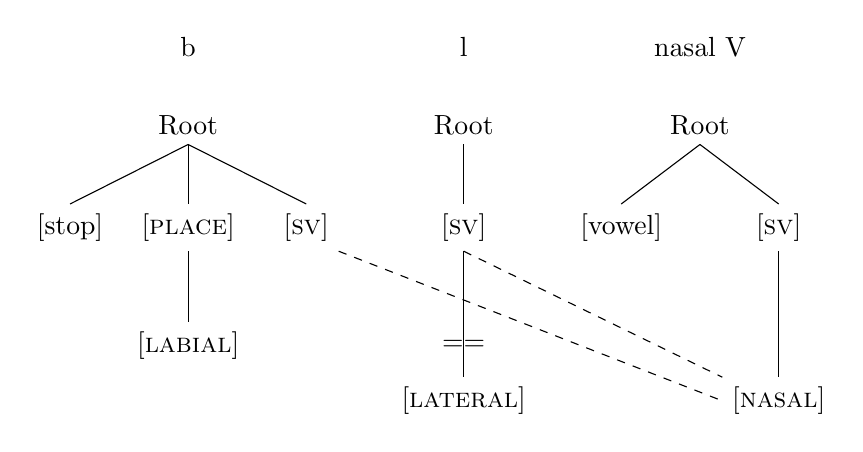
\begin{tikzpicture}
\draw (1.5,0) node {b};
\draw (1.5,-1) node (root) {Root};
\draw (0,-2.3) node (stop) {[stop]};
\draw (1.5,-2.3) node (place) {[\textsc{place}]};
\draw (3,-2.3) node (sv) {[\textsc{sv}]};
\draw (1.5,-3.8) node (labial) {[\textsc{labial}]};
\draw (root.south) -- (stop.north);
\draw (root.south) -- (place.north);
\draw (root.south) -- (sv.north);
\draw (place.south) -- (labial.north);

\draw (5,0) node {l};
\draw (5,-1) node (root2) {Root};
\draw (5,-2.3) node (sv2) {[\textsc{sv}]};
\draw (5,-3.8) node {==};
\draw (5,-4.5) node (lateral) {[\textsc{lateral}]};
\draw (root2.south) -- (sv2.north);
\draw (sv2.south) -- (lateral.north);

\draw (8,0) node {nasal V};
\draw (8,-1) node (root3) {Root};
\draw (7,-2.3) node (vowel) {[vowel]};
\draw (9,-2.3) node (sv3) {[\textsc{sv}]};
\draw (9,-4.5) node (nasal) {[\textsc{nasal}]};
\draw (root3.south) -- (vowel.north);
\draw (root3.south) -- (sv3.north);
\draw (sv3.south) -- (nasal.north);

\draw [dashed] (sv.south east) -- (nasal.west);
\draw [dashed] (sv2.south) -- (nasal.north west);
\end{tikzpicture}

\pagebreak

\ex  {\hspace{1em}}\newline
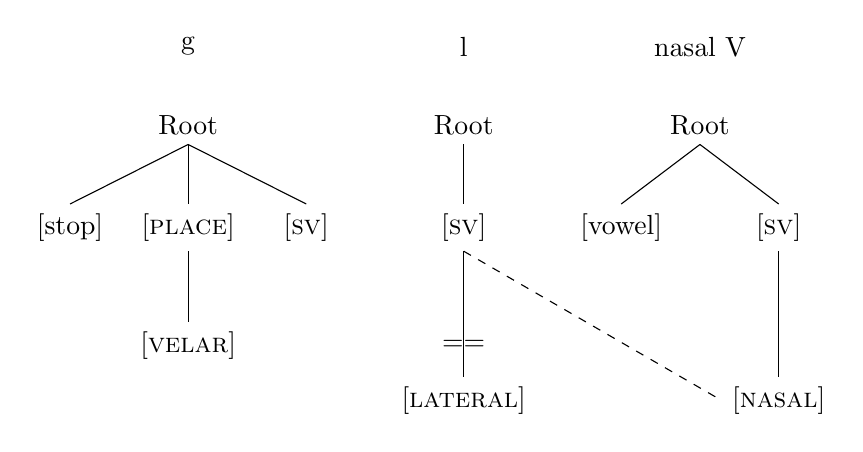
\begin{tikzpicture}
\draw (1.5,0) node {g};
\draw (1.5,-1) node (root) {Root};
\draw (0,-2.3) node (stop) {[stop]};
\draw (1.5,-2.3) node (place) {[\textsc{place}]};
\draw (3,-2.3) node (sv) {[\textsc{sv}]};
\draw (1.5,-3.8) node (labial) {[\textsc{velar}]};
\draw (root.south) -- (stop.north);
\draw (root.south) -- (place.north);
\draw (root.south) -- (sv.north);
\draw (place.south) -- (labial.north);

\draw (5,0) node {l};
\draw (5,-1) node (root2) {Root};
\draw (5,-2.3) node (sv2) {[\textsc{sv}]};
\draw (5,-3.8) node {==};
\draw (5,-4.5) node (lateral) {[\textsc{lateral}]};
\draw (root2.south) -- (sv2.north);
\draw (sv2.south) -- (lateral.north);

\draw (8,0) node {nasal V};
\draw (8,-1) node (root3) {Root};
\draw (7,-2.3) node (vowel) {[vowel]};
\draw (9,-2.3) node (sv3) {[\textsc{sv}]};
\draw (9,-4.5) node (nasal) {[\textsc{nasal}]};
\draw (root3.south) -- (vowel.north);
\draw (root3.south) -- (sv3.north);
\draw (sv3.south) -- (nasal.north);

\draw [dashed] (sv2.south) -- (nasal.west);
\end{tikzpicture}
\end{xlist}
\end{exe}

\subsection{Morpheme-final or coda position\is{coda position}}

If that were the whole story, of course, it would not be very exciting, since under either the old theory or the new one, we have a simple assimilation to describe. However, the other context for [b] and [g] brings up other issues.

We have just established that \ili{Lakota} [b] and [g] in \isi{cluster}s are \isi{sonorant} allophones of /p/ or /ph/ and /k/, so we can now use that discovery to analyze those sounds in morpheme final position. Here the phonological\is{phonology} phenomenon is not assimilation, however --- there is no spreading or copying. Rather, we have a change conditioned by the position of the segment in the word. Let us look a little more closely at exactly what is going on here.

When the underlying final vowel of a morpheme is deleted, the consonant preceding it comes to stand in word or morpheme final position, and at the same time, the syllable structure of the morpheme changes. In the simplest case, what used to be the onset of the final shifts to the coda\is{coda position} of the former preceding syllable, as in these examples ( <.> is a syllable boundary):

\begin{exe}
\ex\label{ex:rood:12} Examples of syllable structure changes when a vowel is lost
\begin{xlist}
\ex \textit{khú.\v{z}a} `be sick' reduplicates \textit{khu\v{s}.khú.\v{z}a}
\ex \textit{\v{s}á.pA} `be dirty' + \textit{yA} `cause' > \textit{\v{s}ab.yÁ}
\ex \textit{\v{s}úŋ.ka} `dog' + \textit{má.ni.tu} `wilderness' > \textit{\v{s}uŋ[ŋ](g).má.ni.tu} `coyote'
\end{xlist}
\end{exe}

In more complicated cases, e.g. when the element following the deleted vowel itself begins with a vowel, the newly final consonant can remain in onset position, and we usually do not see the consonant modification. However, vowel initial words often begin with a phonetic \isi{glottal} stop ([ʔ]), and sometimes that \isi{glottal} stop remains part of the structure of the word in non-initial position. (When or whether the \isi{glottal} stop in this language is a phoneme is an unexplored question, but it often seems to be unpredictable.) Examples of this are found in \REF{ex:rood:13}:

\begin{exe}
\ex \label{ex:rood:13}Varying resyllabification before vowel-initial second elements
\begin{xlist}
\ex \textit{Lak\v{h}\'ota} `\ili{Lakota}' + \textit{iyápi} `language'
\begin{xlist}
  \ex \textit{La.k\v{h}\'ol.ʔi.ya.pi}
\ex \textit{La.k\v{h}\'o.ti.ya.pi}
\end{xlist}
\ex 
\begin{xlist}
\ex \textit{\v{c}haŋ.té} `heart' + \textit{aglé} `set against' > \textit{\v{c}haŋ.tágle} `plot (evil) against'
\ex \textit{\v{c}haŋ.té} `heart' + \textit{ʔasní} `recover' > \textit{\v{c}haŋl.ʔásni} `calm down from an angry spell'
\end{xlist}
\end{xlist}
\end{exe}

The conflicting \isi{glottal}-stop phenomena sometimes result in doublets such as the combination of \textit{Lak\v{h}\'ota} `\ili{Lakota}' plus \textit{iyápi} `language' (see (13a)). In this example, if the \isi{glottal} stop remains in the \isi{compound}, we have the form \textit{La.k\v{h}\'ol.- ʔi.ya.pi}, with /t/ > [l] in \isi{coda position}. However, if the \isi{glottal} stop is omitted in the \isi{compound}, we get the form \textit{La.k\v{h}\'o.ti.ya.pi}, in which the /t/ does not change because it is still in syllable onset position. Both of these constructions are grammatical. A third possibility, illustrated by example (8c) above, \textit{\v{s}uŋ.k'á.kaŋ.yaŋ.ke} `ride horseback', manifests a rule that a voiceless stop followed by a \isi{glottal} stop may merge the two into an \isi{ejective}, which then prevents the change from obstruent to \isi{sonorant}. Which of these three realizations (sonorant-syllable boundary, syllable boundary-voiceless stop, or syllable boundary-\isi{ejective}) is actually used is lexically and perhaps idiolectically conditioned.

Instead of doublets, we sometimes see lexically conditioned constructions with one or the other syllable structure, e.g. (see 13b) \textit{\v{c}haŋ.té} `heart' + \textit{a.glé} `set against' > \textit{\v{c}haŋ.tá.gle} `plot (evil) against' (no \isi{glottal} stop beginning the second element of the \isi{compound}) in contrast with \textit{\v{c}haŋ.té} `heart' + \textit{ʔa.sní} `recover' > \textit{\v{c}haŋl.ʔá.sni} `calm down from an angry spell', in which the /t/ changes its role in the syllable and consequently changes to a \isi{sonorant}.

Phonologists\is{phonology} often discuss changes of this sort using the concepts of segment weakening\is{lenition} or strengthening, also called \isi{lenition} or fortition (but note \citealt[10]{Honeybone2008}): ``Cases of real fortition are vanishingly rare.''). These concepts have been around since the mid-19\textsuperscript{th} century at least (\citealt{Honeybone2008}), but there is often disagreement among scholars as to which contexts are strengthening and which are weakening, or which phonetic phenomena constitute one or the other of those processes. Word final devoicing in \ili{German}, for example, is sometimes argued to be fortition to mark a word boundary (\citealt{IversonSalmons2007} as cited in \citealt{Harris2009}), but much more often described as \isi{lenition} (\citealt{Harris2009}), perhaps as a consequence of vocal tract relaxation at the end of a unit. In support of the latter position in general, not just for \ili{German}, \citet[112]{Szigetvari2008} asserts ``It is a phonological\is{phonology} commonplace that consonant \isi{lenition} is typical in Coda position\is{coda position}.'' Since our target sounds are in \isi{coda position}, we should therefore look for a way to declare their voicing to be \isi{lenition}.

There are numerous definitions of \isi{lenition} in the literature (see \citealt{Honeybone2008}, \citealt{Harris2009}, and \citealt{Szigetvari2008} for discussion). Sometimes it can be described as moving toward a less marked version of the sound, sometimes as the loss of a distinctive feature (which may amount to the same thing), and sometimes it is defined, utilizing a particular sonority hierarchy, as an increase or decrease in sonority, though there is little consensus about which sounds are more \isi{sonorant} than others, especially among the obstruents. Another hypothesis, specifically to explain final devoicing, is that the word boundary has the properties of a voiceless obstruent, so final devoicing is assimilation to the voicelessness of the word boundary.

Obviously, assimilation to the word or morpheme boundary is not available to describe adding [\textsc{voice}] to the \ili{Lakota} stops, and since the change in question adds rather than subtracting a feature, the ``remove a feature'' or ``move toward unmarked'' categorization is also wrong for the stops here, though it does describe the behavior of the fricatives accurately. That leaves us with the idea that the principle in \ili{Lakota} for coda\is{coda position} consonants is ``make them \isi{sonorant}''. \citet[5]{Rankin2001} formulated this as a sound law: syllable final stops become sonorants. He posits that the first version of this \isi{sound change} was to produce nasals in syllable final position, since nasals are the least marked sonorants (cf. \citealt{Rice1993}). Then [b] and [g] result from de-\isi{nasalization} in oral contexts. I do not think we need to posit such a sequence, since we have a theoretical device for directly turning stops into sonorants: add [\textsc{sv}] to the stop. The labial and velar then become \isi{sonorant obstruents}, and the coronals become [l]. The change from [\v{c}] to /g/ requires a change in place as well, but the voicing is now accounted for.

Before we accept this analysis, however, we should take note of another situation where voiced obstruents frequently replace voiceless ones, namely, in intervocalic position. There are many examples of this in the history of the \ili{Romance} languages. Here the process seems to be voicing assimilation, and it is usually called \isi{lenition}. If we carry this description of voiced stops as the result of \isi{lenition} over to word or syllable final position, however, we are faced with a major contradiction: both devoicing, as in \ili{German}, and voicing, as in \ili{Romance}, are called \isi{lenition}. I think we cannot have it both ways, and therefore invoke, again, the concept of [\textsc{sv}] as different from [\textsc{laryngeal voice}]. Loss of [\textsc{laryngeal voice}] (fricatives) and addition of [\textsc{sv}] (producing sonorants from stops) can then both be \isi{lenition}.

Consequently, it seems clear that the combination of analyzing [b] and [g] as sonorants and observing that they are allophones of voiceless and aspirated stops in codas\is{coda position}, an environment that characteristically supports weakening\is{lenition}, is probably the correct description of just what these sounds are doing in this language. The analysis is strengthened by the addition of [l] to the class that includes [b] and [g], since [l] is an underlying \isi{sonorant} to begin with. Using the concepts developed by \citet{Mielke2008}, we can thus describe an ``emergent'' phonological\is{phonology} class for this language consisting of [b,g,l]. Moreover, the fact that all three of these sounds can undergo the further addition of [\textsc{nasal}] means that they must have an [\textsc{sv}] or \isi{sonorant} node to which the feature can spread from the vowel.

As alluded to above, \citet[5]{Rankin2001} came to a similar conclusion using historical reconstruction principles instead of phonological\is{phonology} theory. He isolated the voiced variants of the coda\is{coda position} stops and speculated that there was a \isi{sound change} which turned stops into sonorants, perhaps starting with all of them becoming nasals (the least marked sonorants, according to \citegen{Rice1993} analysis), after which [b] and [g] denasalized\is{nasalization} in non-nasal contexts. He says: 
\begin{quote}It seems clear that [...] [the] stops systematically become/became the corresponding sonorants. This is relatively clear from the inventory of reflexes [...] alone: of these, m, n, ŋ and l are sonorants. Only b and g are stops and phonetic obstruents. But although they are phonetic stops, they have residual voicing left over from their \isi{sonorant} phonological\is{phonology} status. I would claim that, even synchronically, the mysterious voiced stop codas\is{coda position} are actually variants not of the underlying, voiceless stops but of voiced sonorants.\end{quote}

\section{Issues in need of further investigation}

There remain, however, two rather embarrassing complications to this determination, namely the variability in the degree of voicing in the stops in the coda\is{coda position}, and the variability in the \isi{nasalization} in the same context. Furthermore, we have not said anything about the process whereby /y/ becomes [l] in the \isi{sonorant} \isi{cluster}s. All three of these deserve further study, but some hints about how and where to look are available from both theoretical \isi{phonology} and Siouan historical studies.

\subsection{Variable voicing}

The definitions and descriptions of sonorants, including \isi{sonorant obstruents}, in the literature frequently make the point that these sounds are by definition spontaneously voiced, and fully voiced throughout the duration of their articulation.\footnote{Let me remind the reader that what we have for decades been calling voiceless sonorants (e.g. the initial \textit{wh-} in \ili{English} \textit{which} in some \isi{dialects}, or the sound spelled <ll> in \ili{Welsh}) are now considered better described as \isi{sonorant}s with the feature [\textsc{spread glottis}], the same feature that produces aspiration in stops.} Note, for example, that \citet[188]{Botma2011} says of several African languages ``that \isi{sonorant} stops are consistently realized with \textit{active} voice facilitation, and that the degree of voice facilitation is such that these sounds are voiced throughout their duration'' [emphasis in original]. We have seen, however, that this is not the case for \ili{Lakota} [b] and [g]. We have been relying on Rice's\ia{Rice, Keren} determination that the kind of ``voicing'' found in sonorants is phonologically\is{phonology} different from the laryngeal voice found in obstruents, but no one has discovered a phonetic difference in the way voice is physically (phonetically) manifested in these two categories. Yet the case for phonological [\textsc{sv}] is compelling enough that we should not abandon the analysis on the basis of the manifestation of [\textsc{voice}], but rather think about how we might accommodate variable voicing in the analysis.

I propose that the explanation can be derived from the observation that languages can use the voiced/voiceless contrast in two different ways. One recent summary of this proposal is found in \citet[15--19]{Harris2009}, another in \citet{RingenEtAl2013}. They divide languages into ``voicing'' and ``aspiration''\is{aspiration language} types. In voicing languages, like \ili{Dutch} and \ili{French}, there is no Voice Onset Time (VOT) delay after either voiced or voiceless stops in initial position, and the vocal fold vibration accompanying voiced stops is present throughout the duration of the stop closure in both initial and final position unless the language also has a final devoicing rule (\ili{Dutch} does, \ili{French} does not). Final voiced stops may even manifest audible voice after the release of the stop; some refer to that as ``post-voicing''.

In \isi{aspiration language}s, like \ili{German} and \ili{English}, on the other hand, there is a contrast in word initial position between significant VOT delay and its absence. The delay in voice onset is heard as aspiration on the stop. When the stop is not aspirated, phonetic voicing can ``leak'' into it from the environment. It is a commonplace in beginning phonetics classes, for example, to have students observe that a word initial [b] in \ili{English} does not start its voicing immediately at the beginning of the stop closure, and a word-final [b] loses its voicing part way through the closure. Although most of us have been taught that this is assimilative or ``leaking'' voicelessness into an underlyingly voiced consonant, the new analysis is instead that the stops (spelled <b>, <d>, <g>) are not voiced at all in their underlying forms -- this kind of voice is not phonologically significant. What counts for \isi{phonology} is the presence vs. absence of aspiration. Anecdotal evidence for the importance of aspiration over voice in \ili{English} can come from the observation that beginning \ili{English}-speaking phonetics students have to work hard to hear so-called voiceless unaspirated stops\is{simple stops}, transcribing\is{transcription} them as voiced instead. It is clear that \ili{Lakota} is an \isi{aspiration language} in this \isi{typology}, albeit largely without much ``leaking'' of voice into the plain stops\is{simple stops}.

I do not know whether the languages that are cited in support of the [\textsc{sv}] hypothesis are voicing or aspiration, but it seems possible that the determination that \isi{sonorant obstruents} are voiced throughout their duration could correlate with the ``voicing'' \isi{typology}. However, \ili{Lakota} appears to be a language that both has \isi{sonorant obstruents} and is an \isi{aspiration language}. Since the phonetic voice which manifests phonological\is{phonology} [\textsc{sv}] can only come from the environment, the observed variability in the manifestation of that voice makes sense. Evidence for this comes from the informal observation that [b] and [g] in \isi{coda position} often seem to match the voice phonetics of the following consonant. For example, \textit{t\v{h}áŋka} `large' is recorded in the \isi{dictionary} as reduplicating \textit{t\v{h}aŋkt\v{h}áŋka}, but forming the adverb \textit{t\v{h}aŋgyá}. It would seem worthwhile to examine how \isi{sonorant obstruents} are realized in other \isi{aspiration language}s.

\subsection{Variable nasalization\is{nasalization}}

I have not discovered an equivalently neat solution to the nasal variation, but a recent phonetic study of \ili{Lakota} \isi{nasalization} \citep{ScarboroughetalInPress} may provide a clue. The question investigated was how \isi{nasalization} is manifested in \ili{Lakota} vowels under three circumstances: when the surrounding consonants are oral, when the vowel is oral but a neighboring consonant is nasal, and when the vowel is nasal with neighboring nasal consonants. \begin{quote}The study examines the timing and degree patterns of acoustic vowel nasality across contrastive and coarticulatory contexts [...] With respect to patterns within the vowel, in the absence of nasal consonant context, contrastive vowel \isi{nasalization} is generally greatest in degree late in the vowel. Low nasal vowels in carryover contexts parallel this pattern (despite the location of the nasal consonant before the vowel), and low nasal vowels in anticipatory contexts are most nasal at the start of the vowel.\end{quote} \citep{ScarboroughetalInPress}.

Siouanists are convinced that historically, vowel \isi{nasalization} is underlying and nasal consonants are derived when \isi{nasalization} is spread from the vowel \citep{RankinEtAl1998}. This, of course, is also the pattern we have described above for [b] and [g]. In the \isi{sonorant} \isi{cluster}s, the following vowel spreads \isi{nasalization} leftward, including /b/ in its target but excluding /g/; in \isi{coda position}, a preceding nasalized vowel may spread its \isi{nasalization} rightward to varying degrees. In both cases, the phonetic \isi{nasalization} is strongest at the edge of the vowel which is further from the nasal consonant. The historical development is always a leftward spread. Schematically, assuming that the phonetic pattern discovered by \citet{ScarboroughetalInPress} is also the historical one:

\begin{exe}
\ex \label{ex:rood:14}Phonetically gradient nasality in adjacent consonants and vowels
\begin{xlist}
\ex In the \isi{cluster}s and historically for all sonorants:

\begin{tabular}{ c c c c c }
Sonorant(s) & & first part of vowel & & last part of vowel \\
fully nasal & & less nasal & &more nasal \\
&C & & Vŋ \\
\end{tabular}
\ex In the codas\is{coda position}:

\begin{tabular}{ c c c c c c }
Vowel start & & vowel end & C start  & & C end \\
most nasal & & less nasal & most nasal & & less nasal \\
& Vŋ & & & C \\
\end{tabular}
\end{xlist}
\end{exe}

So the \isi{cluster} pattern matches the historical pattern (and there is no ``partially nasal'' in the consonants of the \isi{cluster}s), while in the coda\is{coda position}, the consonant replicates the vowel pattern of decreasing nasality\is{nasalization} during the articulation of the segment. The question to be investigated, then, is whether there is a good explanation for the within-vowel or within-\isi{sonorant} \isi{nasalization} gradient. I leave the answer to future research.

\subsection{The relation between [y] and [l]}

The final topic for this discussion is a mystery that may never be solved, but might inspire someone to try additional research. Throughout the preceding, we have assumed the presence of underlying /l/ in the \isi{cluster}s [bl, gl, gn] and [mn]. However, as was noted briefly above, a very frequent occurrence of these \isi{cluster}s is in conjugated verbs, where [bl] signals first person agent of a verb whose stem begins with /y/, and [gl] represents /k/ in several morphemes, also before a verb stem that begins with /y/.

\citet{Koontz1991} treats the y-initial verbs as one subclass of ``syncopating stems'', reconstructing the [b] as *p and the [g] as *k. We have accounted above for the voicing in the stops, but nothing has been said about a process that could change /y/ to [l] to provide the conditioning environment for the /p/ > [b] and /k/ > [g] phenomena.

The \textit{\isi{Comparative Siouan Dictionary}} \citep{RankinEtAl1998,Rankinetal2015AccessSeptember} point out that proto-Siouan seems to have had five sonorants, which they reconstruct as *r, *y, *w, *R and *W. Informally among themselves, the \isi{dictionary} editors refer to *R and *W as ``funny r'' and ``funny w''. The difference between *r and *R, or between *w and *W, is murky and confusing, since their reflexes are pretty much the same segments (e.g. [l, r, n, d, y, ð], maintaining sonority and coronality for both *r and *R), but distributed differently among the daughter languages. In particular, in \ili{Lakota}, *r descends as /y/, and *R descends as /l/. (For the curious, but irrelevant here, *y descends to \ili{Lakota} as /\v{c}h/). Our [bl] and [gl] \isi{cluster}s, then, are historically *pr and *kr, and somewhere in the more recent history of the language that *r changed to *R in the conjugated forms but remained *r in the stem. No one has made any suggestions about when or how this could have happened, nor exactly what the development might have been. Of little or no additional help, but also in need of an account, is the second person form of these verbs in which the stem-initial /y/ changes to [l] but there is no other prefix.

\section{Conclusion}

We started out to learn about the phonological\is{phonology} status of the phonemically marginal [b] and completely allophonic [g] in \ili{Lakota}. We concluded that they are patterning as sonorants for two reasons: first, because they are assimilating to a following \isi{sonorant}, and only sonorants can acquire an autosegmental\is{autosegmental phonology} feature that would account for them being voiced, and second, because they are sometimes nasal, and only sonorants can be nasals. However, this manifestation of sonority in the obstruents\is{sonorant obstruents} comes from two different directions. On the one hand, both [b] and [g] assimilate (copy) their \isi{sonorant} feature from a following consonant to create \isi{cluster}s, and on the other, [b] and [g], together with [l], constitute a phonological\is{phonology} class that realizes weakening (\isi{lenition}) in \isi{coda position} in derived words. In both patterns, an adjacent nasalized\is{nasalization} vowel can contribute its nasality to the sonorants, but in different ways for each pattern. In the \isi{cluster}s, the conditioning environment follows the \isi{sonorant}, whereas in the codas, it is a preceding nasal that causes the shift. In the codas\is{coda position}, the two stops (but not [l]) show considerable variation in the degree of voicing that they manifest, which may be attributable to the fact that \ili{Lakota} is an \isi{aspiration language} in which obstruent voicing is phonologically\is{phonology} absent and phonetically acquired from the environment. Also in the codas\is{coda position}, the extent to which the \isi{nasalization} feature spreads into the consonants is variable, perhaps repeating the pattern of gradient nasality discovered to be phonetically present in nasalized\is{nasalization} vowels. Finally, we revealed an assimilation problem that takes us into the history of the language, namely the fact that the [l] that we have been studying replaces a /y/ in the verb stem when the verb takes on an agent prefix. That replacement is apparently old, but unexplained.
We have thus combined the phonological\is{phonology} theories of autosegments\is{autosegmental phonology} and \isi{feature geometry}, voicing \isi{typology}, and the history of Siouan to shed light on the question of what the phonological status of the voiced stops is in this language.

\section*{Acknowledgments}

I would like to thank Keren Rice\ia{Rice, Keren} profusely for considerable help with all aspects of this paper, from the inspiration for the analysis to the formatting of rules and examples and suggestions for theoretical bibliography. I have also profited from the comments of an anonymous reviewer, as acknowledged in the appropriate places above, and in addition I would like to thank editor Catherine Rudin\ia{Rudin, Catherine} for very useful feedback.

\section*{Abbreviations}
\begin{tabularx}{.45\textwidth}{lX}
\textsc{neg} & {negation}\\
\textsc{sv} & Sonorant Voice\\
VOT & Voice Onset Time\\
\end{tabularx}


{\sloppy
\printbibliography[heading=subbibliography,notkeyword=this]
 }
\end{document}
